\section{Proposed Algorithm}

\subsection{Proposed ICP Algorithm}

\begin{algorithm}
\caption{Proposed ICP algorithm}
\begin{algorithmic}[1]
\State $\{R_1,t_1\}$ = opticalFlowEstimatedTransf(imageA,imageB)
\State $P_1$ = photoconsistency(A,imageA,B,imageB,$R_1,t_1$)
\State $R=R_1$
\State $t=t_1$
\If $\ P_1 > IDEAL$
    \State $\{R_2,t_2\}$ = SURFestimatedTransf(imageA,imageB)
    \State  $P_2$ = photoconsistency(A,imageA,B,imageB,$R_2,t_2$)
    \If $\ P_2 < P_1$
        \State $R=R_2$
        \State $t=t_2$
    \EndIf
\EndIf
\State A = edgeFilter(A)
\State B = edgeFilter(B)
\State A' $\leftarrow$ transform(A,R,t) 
\State p $\leftarrow$ closestPoints(A',B)
\State $\{R,t\} \gets$ updateTransformation(p)
\State $e_i = meanSquareError(p)$
\If {$e_i < umbral$ OR  $i > maxIterations$} 
	\State return R,t
\Else
	\State goto step 15
\EndIf
\end{algorithmic}
\end{algorithm}


In the first step the proposed algorithm uses optical flow (\ref{sec:oflow}) to obtain a candidate estimation of 
$R,t$ for the first iteration of the ICP algorithm. If the photo-consistency (\ref{sec:photocons}) is bigger than a threshold 
SURF (\ref{sec:surf}) algorithm is applied and the transformation with best photo-consistency is used as input to ICP.

SURF and optical flow work on the 2D image space, but using 
the 3D information from the depth map it is possible to get the 3D position 
of the each pair of correspondences respect to the camera. 

Having pairs of 3D points, points of the frame at time $t$ and corresponding points 
of the frame at time $t + 1$ it is possible to obtain the rotation $R$ and translation $t$
 that minimizes the distances between them. Obtaining an initial guess 
 for ICP. 

A photo-consistency measure is used to compare the quality of the initial estimations of the sensor
 position and orientation. A good estimation of the relative transform between two frames, implies 
a small difference between the first RGB image projected using the relative transform and the second RGB 
image. Using this calculation we can detect if ICP guess is good or not.

After obtaining a first estimation of $R,t$ the two point clouds are filtered using the proposed edge 
filtering method (\ref{alg:edges}) and then the ICP algorithm iterates to find the desired transformation.


\subsection{Complete process}

\begin{figure}[!h]
\begin{center}
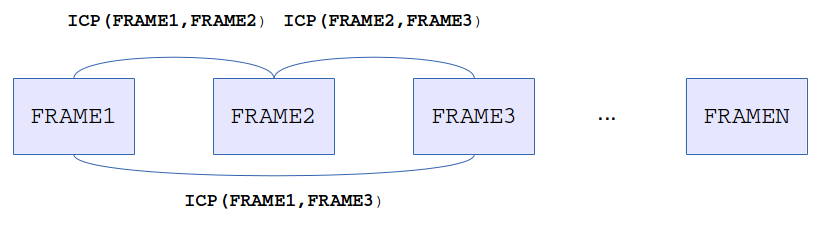
\includegraphics[scale=0.55]{images/graph_icp}
\caption{All constraints are generated by using the proposed ICP algorithm.}
\end{center}
\end{figure}


The complete registration process can be described by the following algorithm:

\begin{algorithm}[H]
\caption{General algorithm}
\begin{algorithmic}[1]
\State read prevFrame
\State globalTransf=4x4MatrixIdentity()
\State addGraphVertex(globalTransf)
\While {read frame} 
\State currentTransf=proposedICP(frame,prevFrame)
\State globalTransf=currentTransf*globalTransf
\State addGraphVertex(globalTransf)
\State addGraphEdge(frame,prevFrame)
\State P = photoconsistency(currentTransf,frame,prevFrame)
\If $\ P > THRESH$
\State index=prevFrameIndex //look for more constraints
\Else
\State index=prevFrameIndex-10
\EndIf
\ForAll {oldFrame in firstFrameIndex to index  } 
\State detectLoopSURF(frame,oldFrame) //check if images are similar
\If {loopDetected}
\State addGraphEdge(frame,oldFrame)
\EndIf
\EndFor
\EndWhile
\State runGraphOptimization()
\end{algorithmic}
\end{algorithm}

\begin{algorithm}[H]
\caption{AddGraphEdge algorithm}
\begin{algorithmic}[1]
\State [R,t] = proposedICP(framei,framej)
\State photoCons = photoConsistency(framei,framej,R,t)
\State informationMatrix=Identity6x6*photoCons;
\State addEdgeToGraph(i,j,R,t,informationMatrix)
\end{algorithmic}
\end{algorithm}
By frame we refer to all the data captured by the sensor (depth map and RGB image).

Consecutive frames are read and then both point clouds are filtered, removing plain surfaces, thus obtaining point clouds 
with a lesser amount of points. With this ICP will work on point clouds that contains around 
only 10\% or 20\% of the original points depending on the scene. But this points are highly representative for registration purposes.

Finally, the classical ICP algorithm is applied to the point clouds.

A graph is generated in the process. Adding spatial restrictions between consecutive frames and also between non-consecutive but similar 
frames. In order to reduce drift with a graph optimization approach \ref{sec:posegraph}, the runGraphOptimization() function 
improves the poses estimated with 
 ICP, using the restrictions generated with addGraphEdge(). 


The graph optimization algorithm internally works with quaternions instead of rotation matrices, as was described in \ref{sec:posegraph}.

